\section{Background}\label{sec:background}

\subsection{Data Source: Censored Planet}

A team of researchers from the University of Michigan presented an overview of
\textit{Censored Planet}, which they term an "internet observatory", at the
\textit{ACM SIGSAC Conference on Computer and Communications Security} in
November 2020~\cite{sundara_raman_censored_2020}. Their automated process scans
the Internet from a number of vantage points around the world using a variety
of protocols.  Each scan runs over a two day period, on average, and produces
millions of records. The Censored Planet data is produced by the Quack and
Hyperquack scans, which scan for keyword blocking at the application layer
using the Echo, Discard, HTTP, and HTTPS internet
protocols~\cite{vandersloot_quack_2018,raman_hyperquack-v1_2020}.

The Echo protocol~\cite{postel_rfc_1983} is the primary transport protocol for
Quack. It is well suited as it is simple and predictable.  An Echo server
listens for and establishes TCP connections, and then returns to the sender any
data that it receives. To detect deep packet inspection based censorship, a
message is sent containing a potentially sensitive keyword, such as a fully
qualified domain for a commonly blocked site. Since an Echo server by design
simply returns the data, if the same Echo server is reachable with one payload
and is not reachable with a different payload from the same location, then
network errors can logically be set aside as the cause for the difference in
behavior; censorship is inferred.  If these same requests are repeated from a
different location to the same server in the same time frame and both requests
find the server reachable from that location, a false determination of
censorship in the unreachable location is not likely. If there is either no
response at all, a response that differs from what was sent, or a network error
code, Quack will repeat the probe to a maximum of 5 attempts. The authors of
Quack assert that this is sufficient to differentiate between network issues
and interference.

A natural response to keyword blocking of HTTP traffic is for users and hosts
to switch to HTTPS. However, the typical TLS exchange to begin encrypted
communication includes the unencrypted fully qualified domain of the requested
server in the opening exchange.~\cite{blake-wilson_transport_2006} Hyperquack
detects keyword blocking of HTTPS traffic by requesting the \textit{incorrect}
server name from previously profiled HTTPS servers maintained by organizations.
The profile created for each target establishes how that endpoint
characteristically sends an error response for requesting a domain not served
by that endpoint.  HyperQuack then requests a domain name that is being tested
for censorship and compares the response.  Responses that differ from the
expected, profiled response indicate possible tampering.  HyperQuack is
therefore able to detect censorship that is particularly targeting HTTPS
traffic.

A sample Quack data record is shown in Figure \ref{example-echo}.  If the probe
receives a response that does not match the template for the query, the result
set also includes a \textit{Response} object which contains the HTTP headers,
the HTTP response code, the body of the response, and any TLS information from
the response.


\begin{figure}[hbt]
\begin{minted}[linenos,tabsize=2,breaklines,fontsize=\footnotesize]{js}
{
  "vp": "114.116.151.108",
  "location": {
    "country_name": "China",
    "country_code": "CN"
  },
  "service": "echo",
  "test_url": "666games.net",
  "response": [
    {
      "matches_template": false,
      "response": "HTTP/1.1 403 Forbidden\nContent-Type: text/html; charset=utf-8\nServer: ADM/2.1.1\nConnection: close\nContent-Length: 520\n\n<html>\n\t<head>\n\t\t<meta http-equiv=\"Content-Type\" content=\"textml;charset=GB2312\" />\n\t\t<style>body{background-color:#FFFFFF}</style> \n\t\t<title>\u975e\u6cd5\u963b\u65ad222</title>\n\t\t<script language=\"javascript\" type=\"text/javascript\">\n         window.onload = function () { \n           document.getElementById(\"mainFrame\").src= \"http://114.115.192.246:9080/error.html\";\n            }\n\t\t</script>   \n\t</head>\n\t<body>\n\t\n\t\t<iframe style=\"width:100%; height:100%;\" id=\"mainFrame\" src=\"\" frameborder=\"0\" scrolling=\"no\"/>\n\t</body>\n</html>\n",
      "start_time": "2021-07-19T01:07:35.692415469-04:00",
      "end_time": "2021-07-19T01:07:37.135588863-04:00"
    },
    {
      "matches_template": false,
      "response": "HTTP/1.1 403 Forbidden\nContent-Type: text/html; charset=utf-8\nServer: ADM/2.1.1\nConnection: close\nContent-Length: 530\n\n<html>\n<head>\n<meta http-equiv=\"Content-Type\" content=\"textml;charset=GB2312\" />\n   <style>body{background-color:#FFFFFF}</style> \n<title>\u975e\u6cd5\u963b\u65ad120</title>\n  <script language=\"javascript\" type=\"text/javascript\">\n         window.onload = function () { \n           document.getElementById(\"mainFrame\").src= \"http://114.115.192.246:9080/error.html\";\n            }\n</script>   \n</head>\n  <body>\n    <iframe style=\"width:100%; height:100%;\" id=\"mainFrame\" src=\"\" frameborder=\"0\" scrolling=\"no\"></iframe>\n    </body>\n      </html>",
      "start_time": "2021-07-19T01:07:42.135655432-04:00",
      "end_time": "2021-07-19T01:07:42.591173508-04:00"
    },
    {
      "matches_template": true,
      "start_time": "2021-07-19T01:07:47.59136423-04:00",
      "end_time": "2021-07-19T01:07:49.284425189-04:00"
    }
  ],
  "anomaly": false,
  "controls_failed": false,
  "stateful_block": false,
  "tag": "2021-07-19T01:01:01"
}
\end{minted}
\caption{Example Quack data record}
\label{example-echo}
\end{figure}

\subsection{Semi-automated Data Analysis}\label{subsec:dataanalysis}
The researchers at Censored Planet have been processing their data using
filtering scripts based on features defined by their knowledge of the
censorship domain. Central to their approach has been a set of "block page
fingerprints" which are strings of text found in the HTML of known block
pages.~\cite{ceccio_censoredplanetcensoredplanet_2021}  Responses are processed
via regular expressions to identify matches with these strings.  This
fingerprint matching process has been the primary means of finding censored
responses.  Recently, the Censored Planet team also began rendering the HTML
response into an image, and using an image classifying neural network,
ResNet50, to cluster responses.~\cite{raman_measuring_2020} They then examine a
sample of each cluster to verify block pages, identify new pages and engineer a
new fingerprint. 

The Censored Planet researchers intentionally chose the image of a block page
for processing through ResNet50 because block pages from the same tool can be
    constructed in various languages.  From the researchers' perspective the
    similarity of visual design allows them to ignore the language of the text.
    However, the deep learning models of Natural Language Processing would open
    the features of the text to be sources of insight. In addition, a visual
    inspection of the page even by a deep learning network does not include any
    data from the headers or other metadata surrounding the request and
    response.

\subsection{Numerical Embeddings from Structured Data}

Once a censored response is discovered, a human expert has to determine what
makes that pattern unique.  That determination must then be condensed to a
regular expression as described in Section~\ref{subsec:dataanalysis}. A
response indicating censorship that is substantially similar can easily be
missed if its differences cause it to pass through the screen of regular
expressions.

Other researchers from the University of Michigan, Armin Sarabi and Mingyan
Liu, presented a method of analyzing structured text data at the \textit{ACM
SIGCOMM Internet Measurement Conference} in
2018~\cite{sarabi_characterizing_2018}. Their demonstration cases used network
intelligence data to detect and predict malicious hosts, as well as to find
hidden host attributes. JSON data was transformed into numeric vectors, or
\textit{vectorized}, and then condensed into what they term \textit{lightweight
numerical embeddings} using a Variational Autoencoder neural network.

A Variational Autoencoder uses two deep learning networks to automate the
encoding of features.  Originally designed for image data, one network encodes
the image to a feature vector.  The second network decodes the vector back to
an image.  The Autoencoder learns to effectively encode the features of the
image by comparing the original with the image produced by the decoder.  Sarabi
and Liu used the \textit{lightweight numerical embeddings} produced by their
Variational Autoencoder as the data source for deep learning analysis on the
original data.

Since the Censored Planet data is structured as JSON, this approach could be
used to gain new insights into censorship or uncover instances of censorship
not previously found in this data. The Censored Planet data also frequently
contains natural language. This approach could be further enhanced using
methods from natural language processing.

\subsubsection{Natural Language Processing Methods for Vectorization and Auto-encoding}

The Censored Planet data contains HTTP responses composed of both typical HTTP
headers and HTML markup of text in multiple languages. This multilingual markup
needs to be vectorized so that our machine learning networks can analyze it. A
team of researchers from Facebook AI Research (FAIR) presented a transformer
based, cross-lingual model to the \textit{Association for Computational
Linguistics} in 2020~\cite{conneau_unsupervised_2020}. They named their model
XLM-R for XLM-RoBERTa as it is a descendent of the
mBERT~\cite{devlin_bert_2019} and XLM~\cite{conneau_cross-lingual_2019} models
developed previously.

A transformer model is built exclusively around the idea of an attention score
which is a weight, or importance value for every item in set B, given a member
of set A~\cite{galassi_attention_2021}.  The attention score is intended to
quantify relevance.  When considering a particular word in the first set, what
are the most relevant words in the second? Figure \ref{fig:atten} shows a
visualization of attention scores for a translation system.  In the figure,
higher scores are represented by lighter squares~\cite{bahdanau_neural_2016}.

\begin{figure}[hbt]
    \centering
    \includegraphics[width=0.8\columnwidth]{../Shawn Duncan M.A. Thesis/attention_example.png}
    % \Description{A rectangular matrix comparing "This will change my future with my family, the man said" to "Cela va changer mon avenir avec ma famille, a dit l'homme" in which the intersection of pairs such as famille & family are white but famille and man are black.}
    \caption{A Visualization of Attention Scores~\cite{bahdanau_neural_2016}}
    \label{fig:atten}
\end{figure}

Transformers use both "self-attention" in which both sets for calculating
attention are the same, such as the input string on itself, as well as
attention between the input and the proposed output. These attention scores are
processed through a standard linear layer to predict the next item of the
output.

The XLM-R model was trained by the team at FAIR using two terabytes of data in
one hundred languages.  The data was taken from Common Crawl which is a
publicly available dataset of text taken from web pages around the
world.~\cite{common_crawl_what_2022} The XLM-R model vectorizes text by
matching a word from any of the languages it recognizes with a numeric token in
its library.

A Sequence-to-Sequence model (Seq2Seq)~\cite{sutskever_sequence_2014} is
composed of an encoder and a decoder. The encoder is presented with each item
in an input sequence, in order, and produces an encoded vector. The decoder
takes the encoded vector as input and produces an output sequence. The primary
use case for a Seq2Seq model is translation.  Imagine that two persons, A and
B, need to communicate but they do not share a language.  Suppose they find two
other persons, encoder and decoder who are both bilingual with exactly one
unknown language in common. Encoder shares a second language with A and decoder
with B.  So person A speaks to encoder, who translates to the unknown shared
language.  Decoder receives the shared translation and translates it again to
deliver it to person B. When a Seq2Seq model is used to build such a
translator, it is trained using supervised learning with pairs of corresponding
phrases.  The Seq2Seq architecture can be used to create an autoencoder if
instead the output sequence is compared back to the input sequence in the
training process.

\subsection{Sequential Data as Images}

Jeyaprakash Hemalatha and an international team of collaborators brought the
tools of computer vision to the task of analyzing sequential data by completely
synthesizing images from the data~\cite{hemalatha_efficient_2021}.  Their
research objective was malware detection.  Grayscale images can be encoded
using a 1 byte pallet, in which the range from black to white is encoded as an
integer between 0 and 255. Figure \ref{fig:parrot} is an example of such an
image. Hemalatha et al. used the bytes of the binary data file to construct a
grayscale image as if the bytes were pixels (Figure \ref{fig:malware}). They
then approached detection as a classification problem and trained a Densenet
based network to classify multiple malware types.

\begin{figure}[htb]
    \centering
    \includegraphics[width=0.45\columnwidth]{../Shawn Duncan M.A. Thesis/Grayscale_8bits_palette_sample_image.png}
    %\Description{A grayscale image of a parrot.}
    \caption{Example grayscale image (1 byte pallet)}
    \label{fig:parrot}
\end{figure}
\begin{figure}[htb]
    \centering
    \includegraphics[width=0.45\columnwidth]{../Shawn Duncan M.A. Thesis/malware.png}
    %\Description{An image that appears to be a randomly distributed collection of pixels of black, white and varying levels of gray.}
    \caption{Malware image constructed from bytes}
    \label{fig:malware}
\end{figure}

The DenseNet architecture is based on the convolutional network architecture
with each convolutional layer receiving not just the prior layer as inputs, but
all prior layers as inputs.~\cite{huang_densely_2017} Although a simple change,
connecting all prior layers prevents gradients from vanishing.  The DenseNet
design is able to match the performance of a much larger standard convolutional
network.  This reduction in model size decreases the computation load resulting
in reduced training time. This design was created for the ImageNet
classification challenge in which each item is sorted into one of 1,000
categories based on the content of the image.~\cite{li_fei-fei_imagenet_2012} 

\section{Research Methodology}\label{sec:research}
\begin{figure}[ht]
    \centering
    \includegraphics[width=\columnwidth]{../Shawn Duncan M.A. Thesis/ma_research.eps}
    \caption{Research Overview}
    \label{fig:process}
\end{figure}
In this thesis we extend the methods of processing structured text with neural networks developed by Sarbani and Liu. First we apply our extended approach to the data provided by the Censored Planet researchers, and then apply supervised learning to select censored responses from the data.  In addition, we compare this approach to fine-tuning a DenseNet to select censored responses from the data encoded as grayscale images.

\subsection{Structured Text to Vectors}\label{subsec:text2vec}
The data coming from Censored Planet is stored as tar archives in Google Cloud
storage. This data needs to be transformed into numeric form before it can be
processed by a machine learning network (see Figure \ref{fig:pre-process}). Our
CensoredPlanetFlatten~\cite{shawn_p_duncan_censored_2022} uses the
Webdataset~\cite{aizman_high_2019} developed by NVIDIA to iterate through the
data streaming directly from the cloud storage. Each item was transformed as it
was received in the stream and stored to local files.  We filtered the stream
to include only items marked as anomalies by the Quack probe, which are
responses that do not match the expected Echo protocol response.

\begin{figure}[hbt]
    \centering
    \includegraphics[width=\columnwidth]{../Shawn Duncan M.A. Thesis/censored_planet_flatten.eps}
    \caption{Vectorizing JSON data}
    \label{fig:pre-process}
\end{figure}

Each result in the source data is structured as nested JSON, the top level is
the metadata common to all the responses for that particular probe, with all
the unique responses nested in the response key (see Figure
\ref{example-echo}). We flattened each record by iteratively pairing the top
level metadata with each set of response data to create a set that pertains to
a single response. Figure \ref{example-flattened} shows an example of two items
flattened from the record shown in Figure \ref{example-echo}.

\begin{figure}
\begin{minted}[linenos,tabsize=2,breaklines,fontsize=\footnotesize]{js}
[{
  "vp": "114.116.151.108",
  "location": {
    "country_name": "China",
    "country_code": "CN"
  },
  "service": "echo",
  "test_url": "666games.net",
  "anomaly": false,
  "controls_failed": false,
  "stateful_block": false,
  "tag": "2021-07-19T01:01:01",
  "matches_template": false,
  "response": "HTTP/1.1 403 Forbidden\nContent-Type: text/html; charset=utf-8\nServer: ADM/2.1.1\nConnection: close\nContent-Length: 520\n\n<html>\n\t<head>\n\t\t<meta http-equiv=\"Content-Type\" content=\"textml;charset=GB2312\" />\n\t\t<style>body{background-color:#FFFFFF}</style> \n\t\t<title>\u975e\u6cd5\u963b\u65ad222</title>\n\t\t<script language=\"javascript\" type=\"text/javascript\">\n         window.onload = function () { \n           document.getElementById(\"mainFrame\").src= \"http://114.115.192.246:9080/error.html\";\n            }\n\t\t</script>   \n\t</head>\n\t<body>\n\t\n\t\t<iframe style=\"width:100%; height:100%;\" id=\"mainFrame\" src=\"\" frameborder=\"0\" scrolling=\"no\"/>\n\t</body>\n</html>\n",
  "start_time": "2021-07-19T01:07:35.692415469-04:00",
  "end_time": "2021-07-19T01:07:37.135588863-04:00"
},
{
  "vp": "114.116.151.108",
  "location": {
    "country_name": "China",
    "country_code": "CN"
  },
  "service": "echo",
  "test_url": "666games.net",
  "anomaly": false,
  "controls_failed": false,
  "stateful_block": false,
  "tag": "2021-07-19T01:01:01",
  "matches_template": false,
  "response": "HTTP/1.1 403 Forbidden\nContent-Type: text/html; charset=utf-8\nServer: ADM/2.1.1\nConnection: close\nContent-Length: 530\n\n<html>\n<head>\n<meta http-equiv=\"Content-Type\" content=\"textml;charset=GB2312\" />\n   <style>body{background-color:#FFFFFF}</style> \n<title>\u975e\u6cd5\u963b\u65ad120</title>\n  <script language=\"javascript\" type=\"text/javascript\">\n         window.onload = function () { \n           document.getElementById(\"mainFrame\").src= \"http://114.115.192.246:9080/error.html\";\n            }\n</script>   \n</head>\n  <body>\n    <iframe style=\"width:100%; height:100%;\" id=\"mainFrame\" src=\"\" frameborder=\"0\" scrolling=\"no\"></iframe>\n    </body>\n      </html>",
  "start_time": "2021-07-19T01:07:42.135655432-04:00",
  "end_time": "2021-07-19T01:07:42.591173508-04:00"
}]
\end{minted}
\caption{Example rows flattened from the data in Figure \ref{example-echo}}
\label{example-flattened}
\end{figure}

Most of the data fields transformed to numbers in a straightforward manner. Datetime fields in ISO format were transformed to UNIX timestamps. Boolean fields transformed to a 1 or 0. We split the IPv4 address into four sequential integers.

There are two text fields needing a more specialized approach: \textit{test\_url} and \textit{response}. This text needs to be transformed to numbers in a consistent and predictable manner. The \textit{response} field is a particular challenge since it can contain the markup of a block page with text in a variety of languages. We used the XLM-R multilingual transformer~\cite{conneau_unsupervised_2020} model to process this text into numeric tokens. Sarbani and Liu term such a transformation \textit{vectorizing}.

Although XLM-R is fast and skilled at vectorizing multilingual text, it requires a token library with just over 250,000 members.  To reduce the scale of training for our autoencoder, we created our own index of the XLM-R tokens being used as we vectorized the data. This reduced the scale of the token vocabulary for our data down to 6,813 active tokens.

\subsection{Training Data}\label{subsec:training}
We used the Censored Planet collection of regular expressions described in Section \ref{subsec:dataanalysis} to determine if an anomalous response was censorship or a false positive~\cite{sarah_laplante_blockpage_2021}. The result was a large dataset of 1,711,339 anomalous responses containing 215,016 censored, 653,481 uncensored, and 842,842 undetermined items. The labeled data is unbalanced since there are 3 times as many responses identified as uncensored as those censored. We applied an approach of under-sampling the majority class to balance the training dataset whenever labeled data was needed.

\subsection{Encoding Features}\label{subsec:encoding}
The majority of the information that comprises a single row in this dataset is natural language in which the sequential relationships are also data. The IP addresses are sequential as well. Once the rows were vectorized into tensors, we trained a Sequence-to-Sequence Autoencoder model to capture the information contained in these relationships~\cite{raff_inside_2021}. The Seq2Seq model is composed of four machine learning blocks: 
\begin{itemize}
    \item Embedding
    \item Encoder
    \item Decoder
    \item Predictor
\end{itemize}

\subsubsection{Embedding}
\begin{table}[h]
  \caption{Embedding Parameters}
  \label{tab:ae_embed}
  \begin{tabular}{p{0.66\columnwidth} r}
    \toprule
    Parameter & \\
    \midrule
    number of embeddings & $7,069$ \\
    embedding dimension & $96$ \\
    \midrule
    trainable parameters &  $6.78 \times 10^{5}$ \\
    \bottomrule
  \end{tabular}
\end{table}
The Embedding block takes token values and creates a tensor to be processed.  It uses 7,069 possible values for input tokens, which is the largest possible value of the static data, 256, added to the 6,813 token values used from XLM-R. We chose an embedding size of 96 to provide sufficient breadth for computation in the processing blocks after experimenting with the impact on memory requirements and processing time using values between 64 and 128.

\subsubsection{Encoder}
\begin{table}[h]
  \caption{Encoder Parameters}
  \label{tab:ae_encoder}
  \begin{tabular}{p{0.66\columnwidth} r}
    \toprule
    Parameter & \\
    \midrule
    input size & $96$ \\
    hidden size & $128$ \\
    \midrule
    trainable parameters &  $1.73 \times 10^{5}$ \\
    \bottomrule
  \end{tabular}
\end{table}
The encoder in our Seq2Seq implementation is a bidirectional Gated Recurrent Unit (GRU) which processes embeddings as a batch, saving each result as a sequence of states. These states are commonly called \textit{hidden states}.  The final hidden state summarizes the entire sequence. When the Seq2Seq model is properly trained, it is this final hidden state from the encoder that will correspond to Sarbani and Liu's \textit{lightweight numerical embeddings}. As a bidirectional GRU, the functional size of the hidden network is doubled.  We selected 128 for the hidden size. This value multiplies through the decoder and the predictor, exploding memory requirements at higher values. 

\subsubsection{Decoder}
\begin{table}[h]
  \caption{Decoder Parameters}
  \label{tab:ae_decoder}
  \begin{tabular}{p{0.66\columnwidth} r}
    \toprule
    Parameter & \\
    \midrule
    input size & $96$ \\
    hidden size & $128$ \\
    cell layers & $1$ \\ 
    \midrule
    trainable parameters &  $2.71 \times 10^{5}$ \\
    \bottomrule
  \end{tabular}
\end{table}
The complexity of the Seq2Seq model is in the decoder. Before processing an input sequence, we use a simplification of scheduled sampling proposed by Raff~\cite{raff_inside_2021} to randomly choose between \textit{auto-regression} and \textit{teacher forcing} to select the inputs for the decoder. The difference between these strategies begins with the second item of the input sequence. If auto-regression has been chosen the inputs will be sampled from the range of the vocabulary using the probabilities produced by the predictor block.  If teacher forcing is chosen, the decoder inputs are the same as the inputs to the encoder. 

The foundation of the decoder is one or more bidirectional Gated Recurrent Unit Cells, which essentially decomposes the standard Gated Recurrent Unit. This decomposition allows us to calculate attention scores after each token in the input sequence is processed through the GRU cells. Attention scores are computed using a dot product
\begin{equation} \label{eq:1}
score(h_t, c) = \frac{h^T_t \cdot c}{\sqrt{H}}
\end{equation}
with values of $h$ taken from the state produced at step $t$ by the encoder, $c$ is the context, or decoder output at step $t$, and $H$ is the input size used for the GRU Cell. We use the attention scores to calculate a weighted context at each step of the decoding process.

\subsubsection{Predictor}
\begin{table}[h]
  \caption{Predictor Parameters}
  \label{tab:ae_predictor}
  \begin{tabular}{p{0.66\columnwidth} r}
    \toprule
    Parameter & \\
    \midrule
    input size & $512$ \\
    hidden size & $256$ \\
    output size & $7,069$ \\ 
    \midrule
    trainable parameters &  $2 \times 10^{6}$ \\
    \bottomrule
  \end{tabular}
\end{table}
The weighted context is concatenated with the output of the decoder block, and the result is processed by the Predictor block to produce a series of probabilities across the range of possible tokens. These probabilities are then used to compute a cross-entropy loss for each step in the decoding process. The summation of these losses for all decoding steps is used as the loss for the current input. 

\subsubsection{Training}
We trained this model using a randomly selected dataset of 1,197,937 items with an additional 171,134 randomly selected items reserved in a validation dataset. The training was conducted on CPU using a batch size of 2 across a cluster of 8 computing nodes, producing an effective batch size of 16. A large amount of data is an asset for a machine learning network but it is also a challenge if the network is computationally expensive to train. We balanced this asset and constraint by randomly selecting 119,794 items from the training set for use on each epoch. The learning rate varied smoothly between 0.003 and 0.0001.  The network was checked against the validation data following each epoch and the results are shown in Figure \ref{fig:ae_val_loss}. 

\begin{figure}[hbt]
    \centering
    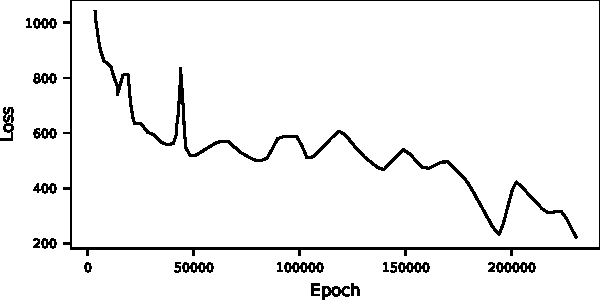
\includegraphics[width=\columnwidth]{../Shawn Duncan M.A. Thesis/autoencoder_val_loss.eps}
    \caption{Sequence-to-Sequence Autoencoder Validation Loss}
    \label{fig:ae_val_loss}
\end{figure}

When a Seq2Seq model is trained for translation, standard practice is to evaluate the quality of the training using a Bilingual Understudy score (BLEU) on both a set of validation pairs and a set of test pairs~\cite{papineni_bleu_2001}. Our Seq2Seq model is not used for translation, therefore we set our training objective as a substantial reduction of accumulated loss. We ultimately evaluate the effectiveness of our Seq2Seq model by its ability to produce \textit{lightweight numerical embeddings} that sufficiently summarize the original data for effective training of the classifier discussed in section \ref{subsec:super}. After our network had seen approximately 3,700,160 items in training, the validation loss had dropped below 0.2 of the initial value, which met our training objective.

We continued by using the trained autoencoder to produce two new datasets from our flattened dataset. We first processed the labeled data through the model, under-sampling the uncensored items, to produce a balanced set of labeled \textit{lightweight numerical embeddings} with 215,016 censored items and 214,846 uncensored items.  We then randomly partitioned this data reserving 0.1 of the data for valdiation, 0.2 for testing and the remaining 0.7 for training. We also processed the undetermined items from our flattened dataset as a set of \textit{lightweight numerical embeddings} for later use as an evaluation dataset.

\subsection{Supervised Learning on Lightweight Embeddings}\label{subsec:super}
\begin{table}[h]
  \caption{Lightweight Embedding Classifier Parameters}
  \label{tab:le_params}
  \begin{tabular}{p{0.66\columnwidth} r}
    \toprule
    Parameter & \\
    \midrule
    initial input & 256 \\
    hidden input & 64 \\
    final input & 32 \\ 
    \midrule
    trainable parameters &  $1.86 \times 10^{4}$ \\
    \bottomrule
  \end{tabular}
\end{table}
The fundamental question for any anomaly identified by the Quack probe is, ``Is this anomaly the result of censorship?'' We construct a binary classifier with three layers: an input layer matching the dimension of the embeddings produced by the autoencoder, a hidden layer which condenses the input, and an output layer that further refines the output of the hidden layer to a probability. We then train this classifier using the balanced labeled dataset of \textit{lightweight numerical embeddings}. The learning rate varied between $1 \times 10^{-6}$ and $1 \times 10^{-7}$ using a cosine annealing strategy with period of 10 epochs.  The results are shown in Figure \ref{fig:le_val_loss} and Figure \ref{fig:le_val_acc}. We use early stopping to prevent the classifier from overtraining as the validation loss drops smoothly through the epochs. The trained network resulted in a loss of $0.047$ on the test data with an accuracy of $0.988$.

\begin{figure}[hbt]
    \centering
    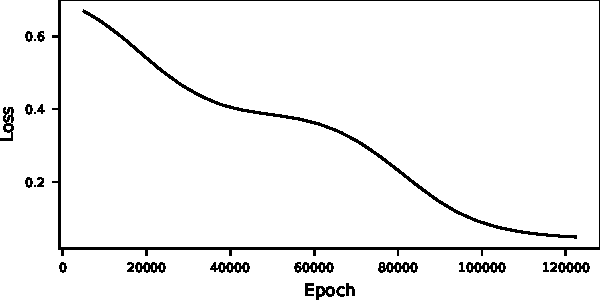
\includegraphics[width=\columnwidth]{../Shawn Duncan M.A. Thesis/le_val_loss.eps}
    \caption{Lightweight Embedding Classifier Validation Loss}
    \label{fig:le_val_loss}
\end{figure}

\begin{figure}[hbt]
    \centering
    \includegraphics[width=\columnwidth]{../Shawn Duncan M.A. Thesis/le_acc.eps}
    \caption{Lightweight Embedding Classifier Validation Accuracy}
    \label{fig:le_val_acc}
\end{figure}

\subsection{Densenet}\label{subsec:dense}
Our original flattened dataset was stored as one dimensional arrays.  We determined that the raw bytes of the largest item would fill a square of size (172, 172).  The Densenet algorithm is well known and available as a pre-trained model that expects images sized (224, 224). We reprocessed the flattened dataset by converting each item to bytes, padding each end of the byte sequence with zeros to produce a $224^2$ length sequence and reshaping the result to (224, 224). We produced two datasets in this manner similar to those produced for the Lightweight Embedding Classifier: a balanced labeled dataset with 215,016 censored items and 215,373 uncensored items, as well as a dataset reprocessed from the 842,842 undetermined items.

The Densenet architecture uses a final linear layer as a classifier for the 1,000 image categories.  We replace that linear layer in the pre-trained model with a new layer accepting the same input dimension but producing a single output.  We then resumed training, fine tuning, the model as a binary classifier. The learning rate varied between $1 \times 10^{-6}$ and $1 \times 10^{-7}$ using a cosine annealing strategy with period of 10 epochs. The results of this training are shown in Figure \ref{fig:dn_val_loss} and Figure \ref{fig:dn_val_acc}. The trained network resulted in a loss of 0.048 on the test data with an accuracy of 0.986.
\begin{figure}[hbt]
    \centering
    \includegraphics[width=\columnwidth]{../Shawn Duncan M.A. Thesis/densenet_val_loss.eps}
    \caption{Densenet Validation Loss}
    \label{fig:dn_val_loss}
\end{figure}

\begin{figure}[hbt]
    \centering
    \includegraphics[width=\columnwidth]{../Shawn Duncan M.A. Thesis/densenet_val_acc.eps}
    \caption{Densenet Validation Accuracy}
    \label{fig:dn_val_acc}
\end{figure}

